\chapter{Introducción}
\label{ch:introduccion}

\section{Contexto}
En los últimos años, la inteligencia artificial (IA) se ha posicionado como una de las herramientas más útiles e interesantes de las que disponemos. El término \textit{<<inteligencia artificial>>} fue acuñado por primera vez por John McCarthy en la Conferencia de Darmouth de 1956~\cite{dartmouth1956}. Años después de que Alan Turing formulase la pregunta sobre si las máquinas podían pensar y plantease el famoso ''Test de Turing''~\cite{turing1950}, varios científicos se reunieron con el objetivo de discutir acerca de la posiblidad de un artefacto de comportarse de manera inteligente. Se llegó a la conclusión de que todo aspecto del aprendizaje se puede describir con tanta precisión que resulte factible construir una máquina que los simule.

La IA se enfoca en crear sistemas que puedan realizar tareas que normalmente requerirían de inteligencia humana. Aunque ha tenido un reciente auge debido a los chatbots o los asistentes personales, presenta una gran cantidad de finalidades. Dentro de los usos que se le dan a la IA destacan la creación y el análisis de productos o la automatización de servicios, además de la optimización de procesos. Esta optimización se enfoca en encontrar la mejor solución posible a un problema dado dentro de un conjunto de opciones factibles. Los algoritmos de optimización y de personalización permiten, por ejemplo, crear aplicaciones que permiten organizar tareas de manera inteligente~\cite{todoist2024} o termostatos que ajustan la calefacción automaticamente~\cite{googlenest2020}.

En el ámbito de la nutrición, la IA tiene un gran potencial para la creación de dietas. La capacidad de analizar grandes volúmenes de datos y entender las necesidades nutricionales de cada paciente permite diseñar planes alimenticios personalizados. No solo cumple con los requisitos calóricos o de nutrientes, sino que también se adapta a los gustos del usuario para tomar en cuenta las preferencias personales o las restricciónes dietéticas.

Este Proyecto Fin de Grado (PFG) se centrará en la resolución de un problema de optimización, la creación de un menú semanal de comidas personalizado que cumpla distintos objetivos, como el número de calorías diarias o la cantidad de macronutrientes ingeridos. Se hará uso de los algoritmos evolutivos, que diseñarán una dieta equilibrada a partir de la selección, cruce y mutación de los distintos alimentos.

Los algoritmos evolutivos son muy útiles para estos problemas de optimización porque permiten explorar una gran cantidad de combinacione posibles para encontrar una solución óptima. El proceso incluye una población inicial de menús, la evaluación de estos según los requisitios nutricionales y la selección de los mejores para la generación de nuevas generaciones mediante cruce y mutación. Este ciclo se repetirá hasta que se obtenga un plan alimenticio optimizado que cumpla con todos los objetivos nutricionales y de preferencia.



\section{Motivación}

La motivación para realizar este proyecto viene dada por el interés creciente en el área de la inteligencia artificial y cómo ha cambiado la manera de plantear los problemas respecto al pasado. En España, el sector TIC (Tecnologías de la Información y la Comunicación) cuenta con más del 40\% de empresas que usan estas herramientas para la automatización de flujos de trabajo, análisis de datos o para la gestión de la cadena de suministro~\cite{ontsi2023}. Buscan mejorar la precisión y la eficiencia a la hora de diseñar soluciones.

No obstante, no solo en sectores tecnológicos se hace uso de la IA. El médico o el alimentario también están incorporándola de manera gradual. Los diagnósticos de imágenes médicas~\cite{philips2024} o la agricultura de precisión~\cite{majeed2024} son cada vez más comunes. También en la nutrición, relacionada con esto ámbitos, estas tecnologías permiten nuevas posibilidades.

\begin{figure}[H]
    \centering
    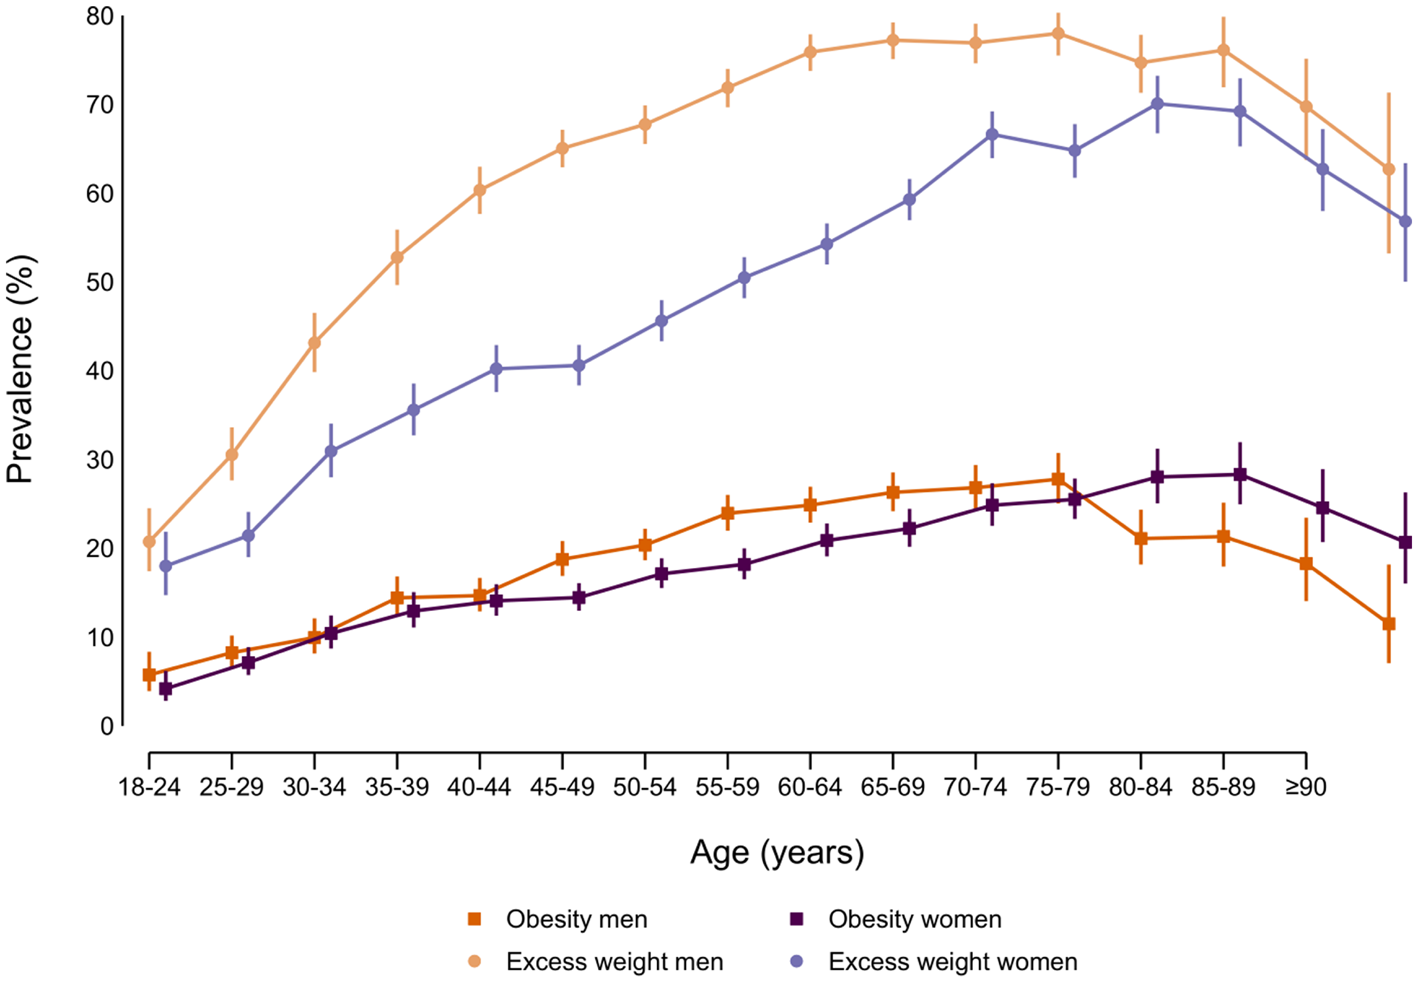
\includegraphics[width=0.75\textwidth]{figures/prevalencia-obesidad.png}
    \caption{Prevalencia (\%) de obesidad y exceso de peso por grupos de sexo y edad. Fuente \cite{ENE-COVID}}
    \label{fig:prevalencia-obesidad}
\end{figure}

Según un estudio llevado a cabo por la \textit{Agencia Española de Seguridad Alimentaria y Nutrición (AESAN)} y por el \textit{Instituto de Salud Carlos III (ISCIII)}, un \textit{55,8\%} de la población adulta española tiene exceso de peso y un \textit{18,7\%} padece obesidad, tal y como se muestra en la figura \ref{fig:prevalencia-obesidad}. Esto trae consigo múltiples problemas de salud, como la aparición de enfermedades crónicas o cardiovasculares, complicaciones respiratorias o dificultades al moverse.

Recientes estudios han demostrado que la IA puede aumentar la adherencia a planes de alimentación saludables un \textit{20\%}, al ofrecer recomendaciones personalizadas y un seguimiento continuo. Además, estas herramientas permiten ajustar dinámicamente las recomendaciones en función de la evolución de la salud del usuario, mejorando así los planes nutricionales~\cite{oh2021systematic}.

La planificación nutricional mediante algoritmos evolutivos ayuda a comprender cómo se pueden mejorar los hábitos alimenticios y la nutrición a través de estas técnicas innovadoras, además de promover una vida sana y bienestar para todos, lo que se relaciona con el tercer objetivo de los Objetivos de Desarrollo Sostenible (ODS)~\cite{ONU2024}, por lo que es un gran aliciente a la hora de realizar este PFG.


\section{Justificación}

En esta sección se deben explicar y argumentar las razones por las cuales se eligió el tema del proyecto, así como su importancia y relevancia. Algunos elementos clave que se pueden abordar en esta sección son:

\begin{enumerate}
    \item \textbf{Relevancia del tema}: ¿Existe alguna necesidad o problema específico que tu proyecto pueda abordar?
    \item \textbf{Justificación teórica}: Mención sobre qué teorías, enfoques o modelos existentes en la literatura respalden la importancia de abordar este tema.
    \item \textbf{Brecha en el conocimiento}: ¿Qué aspectos no se han explorado lo suficiente o no han sido abordados en estudios previos? ¿Cómo puede el proyecto contribuir a cerrar esa brecha en el conocimiento?
    \item \textbf{Contribución práctica}: Aplicaciones del proyecto y cómo pueden beneficiar a la comunidad académica, profesional o a la sociedad en general.
\end{enumerate}

La sección no tiene por qué ser demasiado extensa, ni tiene por qué incluir (o limitarse) a los puntos anteriores, pero debe ser lo suficientemente clara y convincente para que los lectores comprendan por qué el proyecto es relevante y necesario.


\section{Objetivos}
\label{ch:objetivos}

El objetivo general de este proyecto es la creación de una planificación semanal de comidas mediante algoritmos evolutivos. Experimentando con diferentes algoritmos se busca crear un menú que cumpla con distintos objetivos nutricionales, como la ingesta calórica diaria, a la vez que limitarse según las restricciones dadas. Los objetivos específicos de este PFG son:

\begin{itemize}
    \item Desarrollar un algoritmo evolutivo capaz de generar menús que cumplan con las restricciones y los objetivos nutricionales establecidos.
    \item Personalizar el algoritmo para la variación de las comidas según las necesidades específicas de los individuos.
    \item Experimentar con distintas configuraciones y variantes del algoritmo evolutivo en busca de encontrar la mejor solución posible.
    \item Evaluar la sensibilidad y eficacia del algoritmo.
    \item Ejecutar pruebas que validen el algoritmo.
    \item Documentar los resultados obtenidos.
\end{itemize}

\begin{comment}
Una de las partes más importante y complicada. Se considera \textbf{la finalidad} del proyecto en cuestión a realizar y suele encajar dentro de una de las siguientes categorías:

\begin{itemize}
    \item \textbf{Contraste} o validación de una hipótesis. Suele usarse en \glspl{pfm}, no tanto en \glspl{pfg}.
    \item \textbf{Desarrollo} o diseño de algo (e.g.~Software, hardware, sistema, edificio). Suele ser el más común en las ingenierías.
    \item \textbf{Estudio} de un tema que deduce o descubre nuevo conocimiento. Suele ser más común en las ramas de las ciencias puras y humanidades.
\end{itemize}

Sirve como primer indicador de la consecución del proyecto, ya que planteando objetivos podemos determinar en las conclusiones su grado de cumplimiento. Ahora bien, ¿cómo determinamos que un objetivo se ha cumplido? pues definiéndolo para que se pueda cumplir, es decir, intentando que sea:

\begin{itemize}
    \item \textbf{Acotado en el tiempo}, así es más fácil establecer un marco temporal para su realización y programar temporalmente las partes de las que se compone.
    \item \textbf{Medible}, para saber cómo de lejos estamos de llegar a un resultado aceptable.
    \item \textbf{Específico}, de manera que esté bien acotado y sea difícil embarcarse en tareas que no nos acerquen a su consecución.
    \item \textbf{Alcanzable}, porque si no lo es, por mucha intención y esfuerzo que le pongamos no se va a terminar.
    \item \textbf{Relevante}, porque si, en un \gls{pfg} para Ingeniería del Software, desarrollamos un producto mecánico para sexar pollos, pues por muy importante que sea, poco tiene que ver con lo que se ha estudiado durante todos estos años.
\end{itemize}

Regla mnemotécnica: \textit{AMEAR}.
\end{comment}

\section{Estructura de la memoria}

En este subapartado se explicará la estructura del documento.

En el capítulo \ref{ch:estado-arte}, \nameref{ch:estado-arte}, se da un enfoque general al proyecto. Se da contexto sobre las áreas en las que se basa el proyecto: la inteligencia artificial y los algoritmos evolutivos, además de sobre el tema central del PFG, la planificación nutricional mediante algoritmos evolutivos.

En el capítulo \ref{ch:marco-teorico}, \nameref{ch:marco-teorico}, se aporta la base teórica en la que se desarrolla el proyecto. Se indaga en el algoritmo evolutivo y en sus diversas partes, y se explica su funcionamiento.

En el capítulo \ref{ch:desarrollo}, \nameref{ch:desarrollo}, se describe los pasos a seguir para la construcción del algoritmo evolutivo y del planificador de menús, además de la explicación de la base de datos y los conceptos nutricionales necesarios para ello.